\section{Experimental Results and Discussion}

\subsection{Hyperparameter Selection}

For each model, we selected the hyperparameter set 
that achieved the highest average accuracy 
over the 6-fold cross-validation. 

Once the best hyperparameters for each model were 
identified, we employed the Wilcoxon test to determine 
whether the differences between the average accuracies 
of the models were statistically significant. 
This step ensured that the observed differences 
were not due to random variation. 

Finally, we compared the best results obtained from 
the three models (Decision Tree, Random Forest, and Neural Network) 
to assess which model exhibited the 
highest overall performance.

\subsubsection{Decision Tree Results}

As shown in \autoref{tab:dt_search_spaces}, 
the Decision Tree models were evaluated using a 
variety of hyperparameters. The best-performing model, 
Model 2, used the "gini" criterion with a minimum 
impurity decrease of 1e-08 and a maximum depth of 200. 
This combination of hyperparameters resulted in the 
highest average accuracy of 0.3977.

Other models used different criteria and impurity 
thresholds, but none matched the performance of Model 2. 
For example, For example, Model 0 utilized the "gini" 
criterion with a minimum impurity decrease of 0.0 and 
a maximum depth of 200, achieving an average accuracy 
of 0.3954. Model 3, which used the "log\_loss" criterion 
with a minimum impurity decrease of 0.0 and a maximum 
depth of 200, also performed well with an average 
accuracy of 0.3969.

\begin{figure}[H]
    \centering
    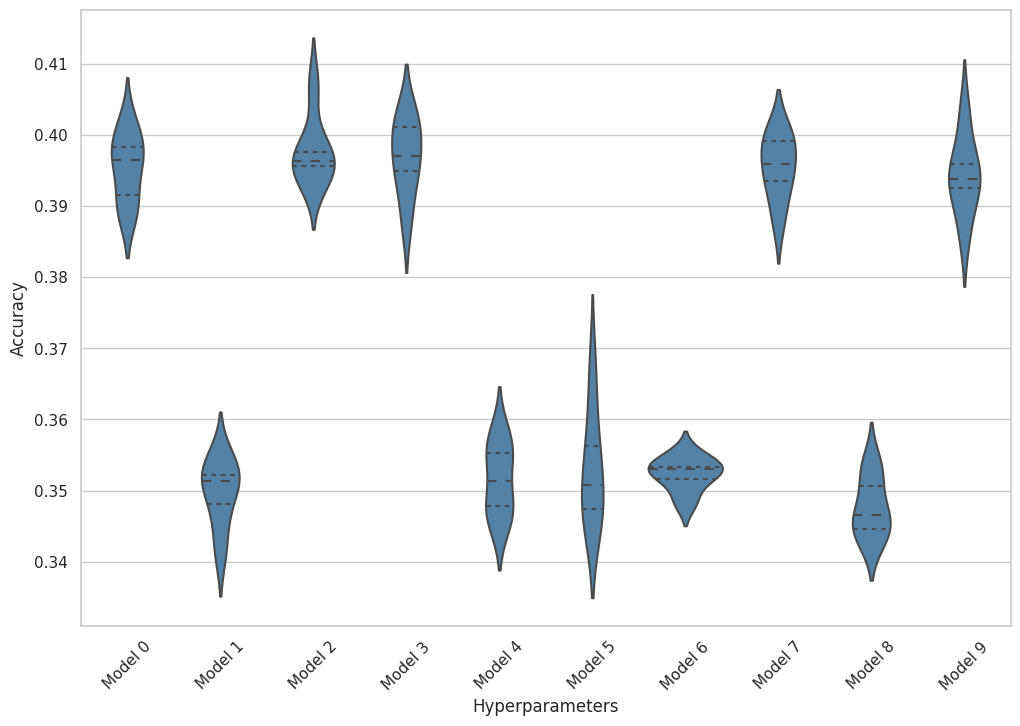
\includegraphics[width=0.99\columnwidth]{images/violin_plot_decision_tree.png}
    \caption{Accuracy distribution for Decision Trees}
    \label{fig:dt_violin_plot}
\end{figure}

The Wilcoxon test results indicate that Model 2 shows 
statistically significant superior performance compared 
to Models 1, 4, 5, 6, and 8, with \( p \)-values below 0.05. 
However, there are no statistically significant differences 
between Model 2 and Models 0, 3, 7, and 9, suggesting 
that their performances are comparable. 
This confirms that Model 2 is among the best, 
but not markedly superior to all the other tested models.

\subsubsection{Random Forest Results}
From \autoref{fig:rf_violin_plot}, it is evident 
that models 1 and 5 performed better than the others. 
Specifically, model 5 achieved the highest performance 
with an average accuracy of 0.5889. 
The accuracy ranged between 0.5819 and 
0.5931, utilizing a configuration of 
150 trees (n\_estimators), 
the "gini" criterion, a minimum impurity decrease of 0.0 and a maximum depth
of 150. Other models demonstrated lower 
performance, with model 2 showing the lowest average 
accuracy of {0.5301}.

The {Wilcoxon test} results indicate that the 
majority of models (0, 2, 3, 4, 6, 7, 8, 9) exhibit 
{p-values} of {0.03125}, confirming a 
statistically significant difference when compared to 
the best model (index 5). Model 1, however, had a \( p \)-value
of {0.4375}, suggesting no significant difference 
in performance compared to the best-performing model.

\begin{figure}[H]
    \centering
    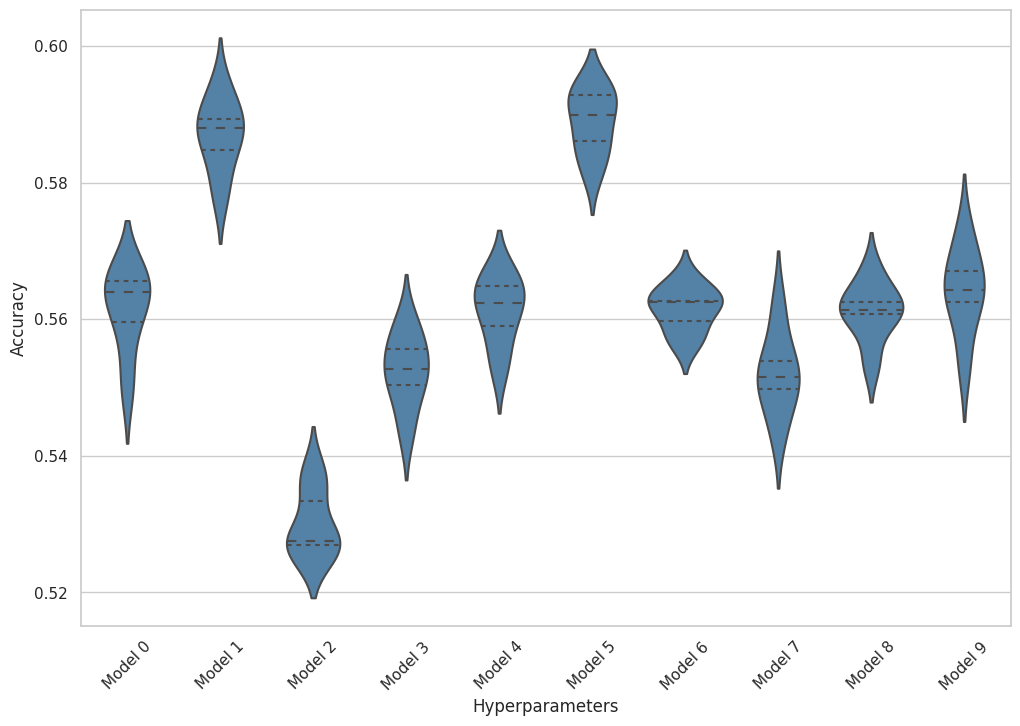
\includegraphics[width=0.99\columnwidth]{images/violin_plot_random_forest.png}
    \caption{Accuracy distribution for Random Forests}
    \label{fig:rf_violin_plot}
\end{figure}

\subsubsection{Neural Network Results}

For the Neural Network models, the detailed results 
are illustrated in \autoref{fig:nn_violin_plot}. 
Model 2 demonstrated the highest performance with 
an average accuracy of 0.5894. This model was configured 
with a hidden size of 64, a learning rate of 0.0005, 
and trained for 8 epochs. The accuracy of Model 2 
ranged from 0.5835 to 0.5943.

The Wilcoxon test results indicate that 
Models 0, 1, 4, 5, and 7 have p-values of 0.03125, 
indicating statistically significant differences 
from Model 2. Model 3, with a p-value of 0.15625, 
shows a less significant difference, and 
Models 6, 8, and 9, with p-values of 0.0625 and 0.09375, 
respectively, also demonstrate less pronounced 
differences. This analysis highlights Model 2 as 
the top performer, with several other models 
showing statistically significant, though lesser, 
performance differences.


\begin{figure}[H]
    \centering
    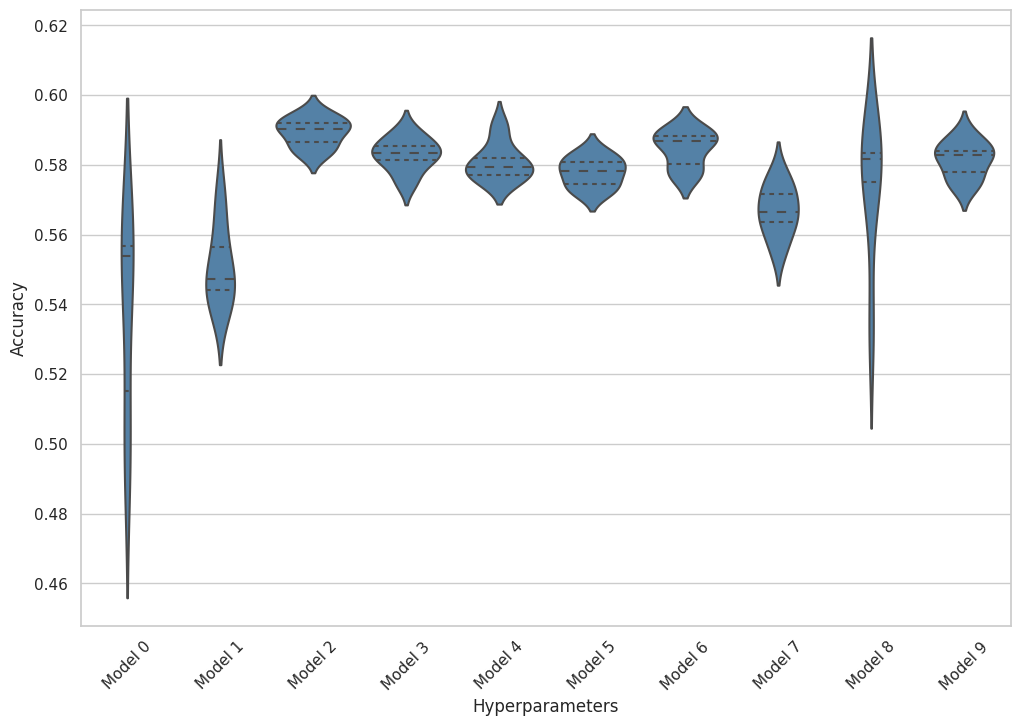
\includegraphics[width=0.99\columnwidth]{images/violin_plot_neural_network.png}
    \caption{Accuracy distribution for Neural Network}
    \label{fig:nn_violin_plot}
\end{figure}

\begin{table*}
    \centering
    \begin{tabular}{@{}cccc@{}}
        \toprule
        \textbf{Index} & \textbf{Criterion} & \textbf{Min Impurity Decrease} & \textbf{Max Depth} \\ \midrule
        0 & gini & 1e-10 & 200 \\
        1 & log\_loss & 1e-08 & 200 \\
        2 & gini & 1e-08 & 200 \\
        3 & gini & 1e-08 & 150 \\
        4 & log\_loss & 1e-10 & None \\
        5 & log\_loss & 0.0 & 150 \\
        6 & log\_loss & 0.0 & None \\
        7 & gini & 1e-10 & 150 \\
        8 & log\_loss & 1e-12 & 200 \\
        9 & gini & 0.0 & 200 \\ \bottomrule
    \end{tabular}
    \caption{Hyperparameters for Decision Tree}
    \label{tab:dt_search_spaces}
\end{table*}


\begin{table*}
    \centering
    \begin{tabular}{@{}ccccc@{}}
        \toprule
        \textbf{Index} & \textbf{Estimators} & \textbf{Criterion} & \textbf{Min Impurity Decrease} & \textbf{Max Depth} \\ \midrule
        0 & 50 & gini & 0.0 & None \\
        1 & 150 & gini & 0.0 & 200 \\
        2 & 50 & log\_loss & 1e-12 & 150 \\
        3 & 100 & log\_loss & 0.0 & 200 \\
        4 & 150 & log\_loss & 0.0 & 150 \\
        5 & 150 & gini & 0.0 & 150 \\
        6 & 150 & log\_loss & 1e-12 & 150 \\
        7 & 100 & log\_loss & 1e-12 & 150 \\
        8 & 50 & gini & 0.0 & 200 \\
        9 & 50 & gini & 1e-10 & 150 \\ \bottomrule
    \end{tabular}
    \caption{Hyperparameters for Random Forest}
    \label{tab:rf_search_spaces}
\end{table*}

\begin{table*}
    \centering
    \begin{tabular}{@{}ccccc@{}}
        \toprule
        \textbf{Index} & \textbf{Hidden Size} & \textbf{Epochs} & \textbf{Learning Rate} \\ \midrule
        0 & 16 & 8 & 0.0005 \\
        1 & 16 & 10 & 0.001 \\
        2 & 64 & 8 & 0.0005 \\
        3 & 32 & 6 & 0.0005 \\
        4 & 64 & 6 & 0.001 \\
        5 & 64 & 8 & 0.001 \\
        6 & 64 & 10 & 0.0005 \\
        7 & 64 & 6 & 0.005 \\
        8 & 32 & 6 & 0.001 \\
        9 & 32 & 10 & 0.0005 \\ \bottomrule
    \end{tabular}
    \caption{Hyperparameters for Neural Network}
    \label{tab:nn_search_spaces}
\end{table*}


\subsection{Best Models Comparison}
The performance of the models, as shown in \autoref{fig:best_models_comparison}, 
reveals that the Neural Network (NN) achieved 
the highest accuracy on both validation and test 
datasets. The NN model reached a validation 
accuracy of 0.5894 and a test accuracy of 0.5996. 
The Random Forest (RF) followed, with a validation 
accuracy of 0.5889 and a test accuracy of 0.5925. 
The Decision Tree (DT) model had the lowest 
performance, with a validation accuracy of 0.3977 
and a test accuracy of 0.3987.

The Wilcoxon test further confirms these observations. 
The test result for the DT model against the NN model 
shows a p-value of 0.03125, indicating a statistically 
significant difference in performance, with the 
DT model performing worse. Conversely, the RF model 
had a p-value of 1.0 when compared to the NN, 
suggesting no statistically significant difference 
in performance between RF and NN. This reinforces 
that while both RF and NN perform comparably, the 
NN model has a slight advantage. Hence, the NN model 
is identified as the best-performing model in this 
comparison.

\begin{figure}[H]
    \centering
    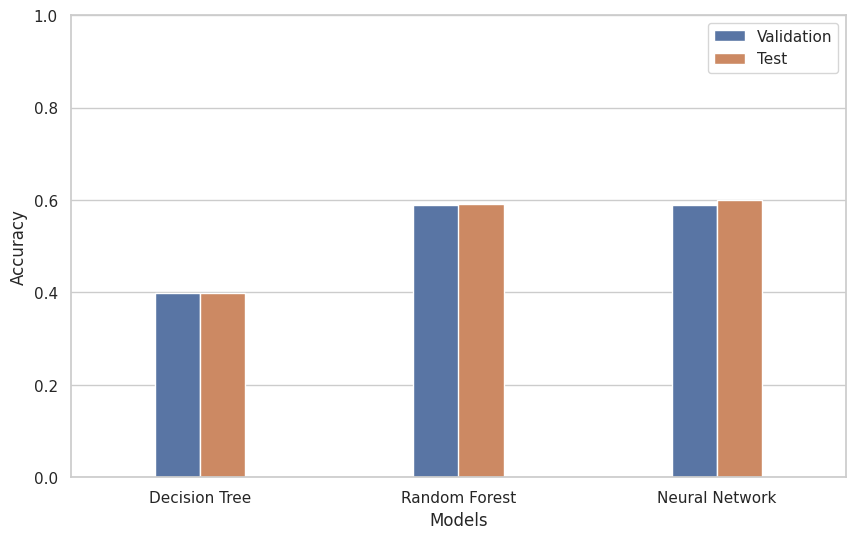
\includegraphics[width=0.99\columnwidth]{images/best_model_test_results.png}
    \caption{Best Models Comparison}
    \label{fig:best_models_comparison}
\end{figure}

\begin{figure*}
    \centering
    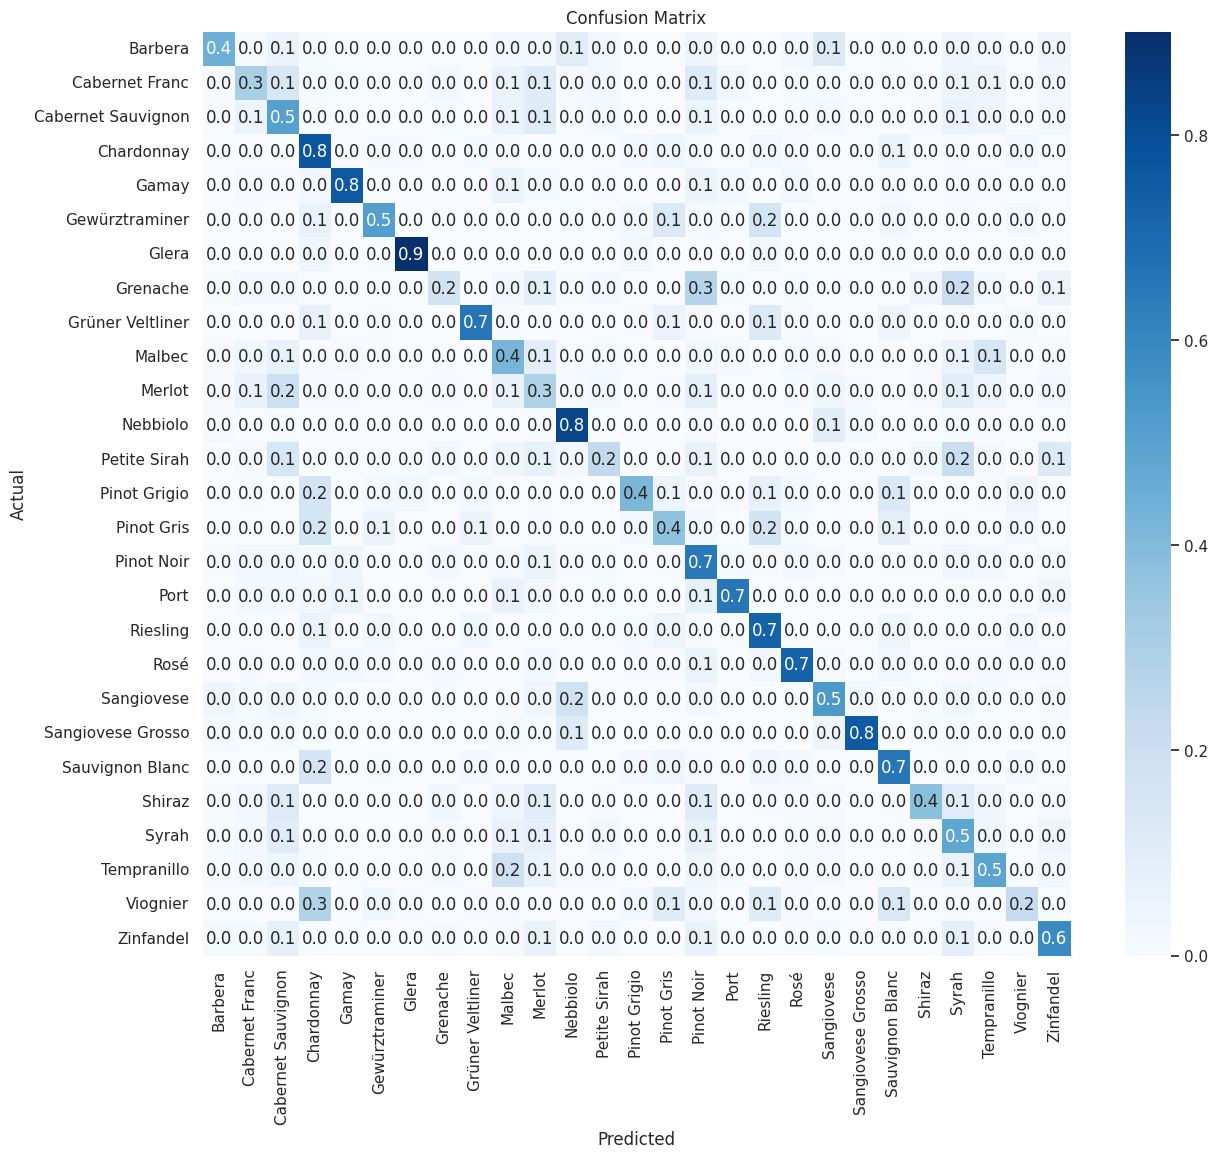
\includegraphics[width=0.99\textwidth]{images/neural_network_confusion_matrix.png}
    \caption{Neural Network Confusion Matrix}
    \label{fig:nn_confusion_matrix}
\end{figure*}

\subsection{Discussion of Results}

The results of this analysis highlight the superior
 performance of the Neural Network model compared 
 to both the Decision Tree and Random Forest models. 
 With the highest validation and test accuracies, 
 0.5894 and 0.5996 respectively, the Neural Network 
 demonstrated its ability to generalize better to 
 unseen data. The confusion matrix in \autoref{fig:nn_confusion_matrix} 
 further supports these findings, showing a 
 concentration of correct predictions along the 
 diagonal, indicating strong classification 
 capabilities across the categories.